% Created by tikzDevice version 0.12 on 2018-11-30 19:07:14
% !TEX encoding = UTF-8 Unicode

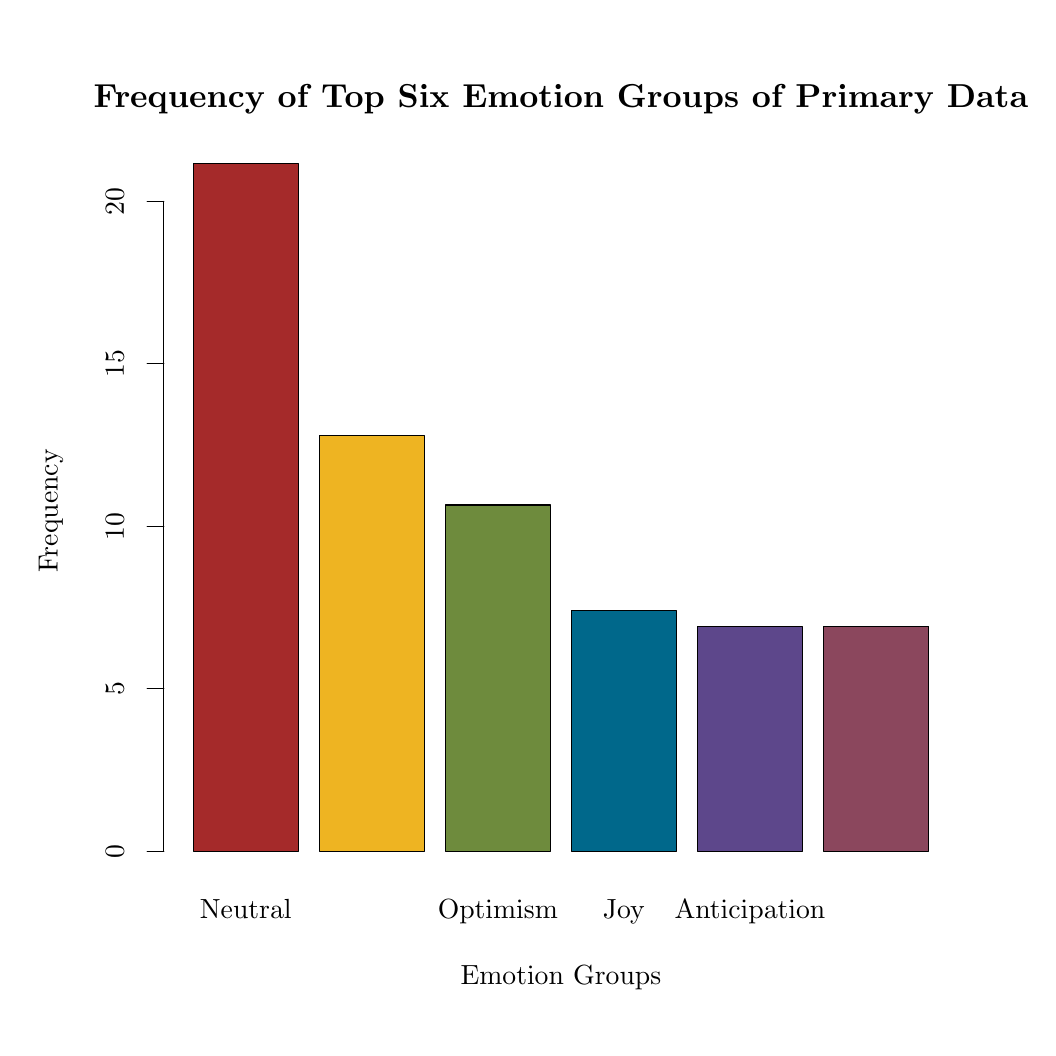
\begin{tikzpicture}[x=1pt,y=1pt]
\definecolor{fillColor}{RGB}{255,255,255}
\path[use as bounding box,fill=fillColor,fill opacity=0.00] (0,0) rectangle (361.35,361.35);
\begin{scope}
\path[clip] (  0.00,  0.00) rectangle (361.35,361.35);
\definecolor{drawColor}{RGB}{0,0,0}
\definecolor{fillColor}{RGB}{165,42,42}

\path[draw=drawColor,line width= 0.4pt,line join=round,line cap=round,fill=fillColor] ( 59.83, 63.68) rectangle ( 97.78,312.15);
\definecolor{fillColor}{RGB}{238,180,34}

\path[draw=drawColor,line width= 0.4pt,line join=round,line cap=round,fill=fillColor] (105.38, 63.68) rectangle (143.33,213.97);
\definecolor{fillColor}{RGB}{110,139,61}

\path[draw=drawColor,line width= 0.4pt,line join=round,line cap=round,fill=fillColor] (150.92, 63.68) rectangle (188.88,188.85);
\definecolor{fillColor}{RGB}{0,104,139}

\path[draw=drawColor,line width= 0.4pt,line join=round,line cap=round,fill=fillColor] (196.47, 63.68) rectangle (234.43,150.69);
\definecolor{fillColor}{RGB}{93,71,139}

\path[draw=drawColor,line width= 0.4pt,line join=round,line cap=round,fill=fillColor] (242.02, 63.68) rectangle (279.97,145.11);
\definecolor{fillColor}{RGB}{139,71,93}

\path[draw=drawColor,line width= 0.4pt,line join=round,line cap=round,fill=fillColor] (287.57, 63.68) rectangle (325.52,145.11);
\end{scope}
\begin{scope}
\path[clip] (  0.00,  0.00) rectangle (361.35,361.35);
\definecolor{drawColor}{RGB}{0,0,0}

\node[text=drawColor,anchor=base,inner sep=0pt, outer sep=0pt, scale=  1.00] at ( 78.81, 39.60) {Neutral};

\node[text=drawColor,anchor=base,inner sep=0pt, outer sep=0pt, scale=  1.00] at (169.90, 39.60) {Optimism};

\node[text=drawColor,anchor=base,inner sep=0pt, outer sep=0pt, scale=  1.00] at (215.45, 39.60) {Joy};

\node[text=drawColor,anchor=base,inner sep=0pt, outer sep=0pt, scale=  1.00] at (261.00, 39.60) {Anticipation};
\end{scope}
\begin{scope}
\path[clip] (  0.00,  0.00) rectangle (361.35,361.35);
\definecolor{drawColor}{RGB}{0,0,0}

\node[text=drawColor,anchor=base,inner sep=0pt, outer sep=0pt, scale=  1.20] at (192.68,332.61) {\bfseries Frequency of Top Six Emotion Groups of Primary Data};

\node[text=drawColor,anchor=base,inner sep=0pt, outer sep=0pt, scale=  1.00] at (192.68, 15.60) {Emotion Groups};

\node[text=drawColor,rotate= 90.00,anchor=base,inner sep=0pt, outer sep=0pt, scale=  1.00] at ( 10.80,186.67) {Frequency};
\end{scope}
\begin{scope}
\path[clip] (  0.00,  0.00) rectangle (361.35,361.35);
\definecolor{drawColor}{RGB}{0,0,0}

\path[draw=drawColor,line width= 0.4pt,line join=round,line cap=round] ( 49.20, 63.68) -- ( 49.20,298.56);

\path[draw=drawColor,line width= 0.4pt,line join=round,line cap=round] ( 49.20, 63.68) -- ( 43.20, 63.68);

\path[draw=drawColor,line width= 0.4pt,line join=round,line cap=round] ( 49.20,122.40) -- ( 43.20,122.40);

\path[draw=drawColor,line width= 0.4pt,line join=round,line cap=round] ( 49.20,181.12) -- ( 43.20,181.12);

\path[draw=drawColor,line width= 0.4pt,line join=round,line cap=round] ( 49.20,239.84) -- ( 43.20,239.84);

\path[draw=drawColor,line width= 0.4pt,line join=round,line cap=round] ( 49.20,298.56) -- ( 43.20,298.56);

\node[text=drawColor,rotate= 90.00,anchor=base,inner sep=0pt, outer sep=0pt, scale=  1.00] at ( 34.80, 63.68) {0};

\node[text=drawColor,rotate= 90.00,anchor=base,inner sep=0pt, outer sep=0pt, scale=  1.00] at ( 34.80,122.40) {5};

\node[text=drawColor,rotate= 90.00,anchor=base,inner sep=0pt, outer sep=0pt, scale=  1.00] at ( 34.80,181.12) {10};

\node[text=drawColor,rotate= 90.00,anchor=base,inner sep=0pt, outer sep=0pt, scale=  1.00] at ( 34.80,239.84) {15};

\node[text=drawColor,rotate= 90.00,anchor=base,inner sep=0pt, outer sep=0pt, scale=  1.00] at ( 34.80,298.56) {20};
\end{scope}
\end{tikzpicture}


